\documentclass{article}
\usepackage[hidelinks]{hyperref}
\usepackage{apacite}
\usepackage{graphicx}
\usepackage{a4wide}
\bibliographystyle{apacite}

\title{Metagenomic Binning Pipelines - the State of the Art}
\author{Theo Portlock}
\begin{document}
\maketitle

\section{Abstract}
\begin{itemize}
	\item \emph{Decision tree graphical abstract for the choice of binning algorithm}
	\item \emph{Features that distinguish binning algorithms}
	\item \emph{Some guidelines for chosing the correct binning techniques appropriate for a given study}
\end{itemize}
New generations of sequencing platforms coupled to numerous bioinformatics tools have led to rapid technological progress in metagenomics and metatranscriptomics to investigate complex microorganism communities.
Nevertheless, a combination of different bioinformatic tools remains necessary to draw conclusions out of microbiota studies.
As sequencing costs have dropped at a rate above 'Moore's law', bigger data sets are available, and proportional costs of analysis have risen as a consequence.
Binning is the grouping of assembled metagenomic contigs by their genome of origin.
Algorithms for binning are a rapidly evolving field.
The number of these algorithms are growing over time.
Selecting the most appropriate binning algorithm can be a daunting task and is influenced on computational resources available and experimental variables relating to the sequencing.
This review serves as a roadmap to direct the reserarcher to the binning algorithm that best suits their needs.

\section{Background}
\begin{itemize}
	\item \emph{General introduction to history of binning}
	\item \emph{increase in popularity of the field of metagenomics}
\end{itemize}
\subsection{History of binning}
Compared to amplicon, shotgun metagenome can provide functional gene profiles directly and reach a much higher resolution of taxonomic annotation.
However, due to the large amount of data, the fact that most software is only available for Linux systems, and the large amount of computing resources are needed to perform analysis...
After collection, the steps involved in preparing the sequencing data for metagenomic analysis are quality control, filtering, and trimming.
Sequence alignment - Bowtie2, Tophat2, Hisat2 are used to map reads against a database
Classifying taxonomy and Annotation - Binning
Binning pipelines: Kaiju, Kraken2, Braken, mOTU, fetchMG, metaphlan, Centrifuge, METEOR, MetaBAT
Galaxy
EBI Metagenomics (MGnify) has doubled the number of publicly available anaysed datasets held within the resource in two years.
orgnaisms have similar tetranucleotide frequencies put contigs together into genome
Spades
tools for binning - Concoct, metabat, groupm, and crAss

\section{Factors to concider before chosing a binning algorithm}
Resource management
Tradeoff between number of CPU's, memory, and time are important conciderations.
Depends on the resources you have available and the required accuracy.
Pipeline vs standalone?
Alignement based or alignment free
An analysis pipeline is defined as a program that combines several softwaare programs in a defined order to complete a complex analysis.
Improperly developed, validated, and/or monitored pipelines may generate inaccurate results. 
	
\section{Methods for metagenomic binning}
\subsection{Metagenome Assembled Genomes}
Viral, environmental, gut, long/short reading, computational,lab resourses etc - deep coverage, how did you recover the sequences, oxford nanopore vs illumina, shotgun vs 16s, number of samples? data preparation before binning, gene orientation, webserver vs local vs supercomuter, competency with the linux environment? sequence coverage, methylation signatures
\begin{figure}
\centering
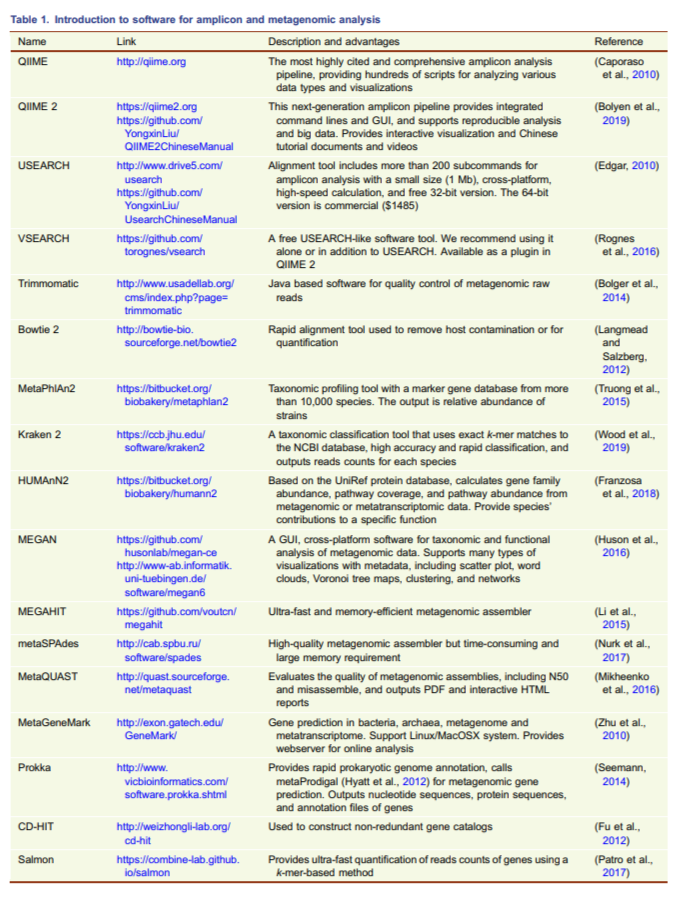
\includegraphics[scale=0.7]{figures/table.png}
\caption[Current pipelines available for metagenomic analysis]{
	Current pipelines available for metagenomic analysis - Something like this? from a 2017 review}
\label{Fpipelines}
\end{figure}

\subsection{Metagenomic Species Pan-genomes}
\subsection{Megagenome Assembled Genome}

\section{Binning microbial genomes with deep learning}
\begin{itemize}
	\item \emph{Not sure if to focus on this or the appropriateness}
	\item \emph{HMP and other }
	\item \emph{The increased impact of machine learning in analysis}
	\item \emph{Short section - just for past-present-future completeness}
\end{itemize}
supervised vs unsupervised
\subsubsection{VAMB}
The integration of deep learning techniques into the field of metagenomics has revolutionised the field of metagenomics.
The VAMB pipeline was developed to take advantage of variational autoencoders; a generative machine learning model that uses a combination 
Improved metagenome binning and assembly using deep variational autoencoders
Nature biotechnology - 4th Jan 2021
the VAMB pipeline \cite{nissenimproved}
\subsubsection{Phylopythia}
\subsubsection{Coconet}

\section{Chosing the most appropriate binning algorithm}
\subsection{Binning for viral genomes}
New insights from uncultivated genomes of the global human gut microbiome
Nature - 13th March 2019 \cite{nayfach2019new}

\subsection{Binning for viral genomes}

\section{Conclusion}
\begin{itemize}
	\item \emph{New and open areas of research in which the application of metagenomic pipelines are relevant}
	\item \emph{HMP and other }
	\item \emph{The increased impact of machine learning in analysis}
	\item \emph{Short section - just for past-present-future completeness}
	\item \emph{Future developments for metagenomic analysis}
\end{itemize}

\section{Notes}
Make a table with the following software:
\begin{itemize}
	\item \emph{MSPminer}
	\item \emph{METEOR}
	\item \emph{VAMB}
	\item \emph{Metaphlan}
	\item \emph{MGnify}
	\item \emph{metabat}
	\item \emph{cocacola}
	\item \emph{NF-core-mag}
\end{itemize}
A review on the benchmarking binning algorithms was done by \citeNP{yue2020evaluating}.

\bibliography{library}
\end{document}

